\documentclass[12pt,a4paper]{article}

\usepackage{graphicx}
\usepackage[latin1]{inputenc}
\usepackage{amsmath}
\usepackage{amsfonts}
\usepackage{amssymb}
\usepackage{graphicx}
\usepackage{caption}
\usepackage{subcaption}
\usepackage{dsfont}
\usepackage{multirow}
%\usepackage[dvips]{color}
\usepackage{color}
%\input{psfig.sty}
\usepackage{natbib}
%\usepackage{cite}
\begin{document}
\begin{itemize}
\item n -- number of cells
\item $J$ -- number of genes
\end{itemize}

Current model:
\begin{eqnarray*}
&&\log(M)=X_M*\alpha_M+U*V\\
&&logit(\Pi)=X_{\Pi}*\alpha_{\Pi}+U*W
\end{eqnarray*}
\begin{itemize}
\item $M$ is $n\times J$ matrix. $M_{ij}$ is the mean parameter for the NB distribution describing the expression of gene $j$ in cell $i$
\item $\Pi$ is $n\times J$ matrix of dropout probabilities
\item $X_M$ is the known $n\times kx_M$ design matrix for the negative binomial part regression.
\item $X_{\Pi}$ is the known $n\times kx_\Pi$ design matrix for the logistic regression.
\item $U$ is the unknown $n\times p$ matrix of latent factors affecting both $M$ and $\Pi$ but with different coefficients (resp. $V$ and $W$)
\end{itemize}
Parameters to estimate are $\alpha_M$, $\alpha_\Pi$, $U$, $W$ and $\theta_j$ (gene-specific (at least for the moment) dispersion parameters for $j=1,\ldots,J$). 

\bigskip
\noindent
The supposed method to estimate parameters: 
\begin{enumerate}
\item Initialize all unknown parameters (with PCA or RUV?)
\item Alternate between two steps:
\begin{itemize}
\item All left hand sides are fixed, estimate right hand sides by maximum likelihood
\item All right hand sides are fixed, estimate $U$ by maximum likelihood
\end{itemize}
\end{enumerate}

\bigskip
\noindent {\bf Where we are:}

\bigskip
\noindent There are codes for each of the steps separately and the one which puts two steps together.

\bigskip
\noindent When tested, two steps together did not work

\bigskip
\noindent Code was put in a form of R package (by JP) where I cleaned up the file functions$\_$svetlana.R which currently contains likelihood functions and gradient functions for each of 
the two steps. I also added the descriptions of parameters.

\bigskip
\noindent  To debug code, I compared the output of my code for the first step (optimization wrt "right parts") with the output of pscl, U being fixed equal to its true value which was used to simulate data.

\bigskip
\noindent  The outputs are the same (as expected because the first step with known $U$ is basically the same thing that the pscl implementation)

\bigskip
\noindent  I did some numerical experiences with this first step optimization in order to see how stable is it and how it depends on the sample size $n$ (optimization is done gene by gene, so the sample size is the number of cells $n$).

\begin{tabular}{ccc}
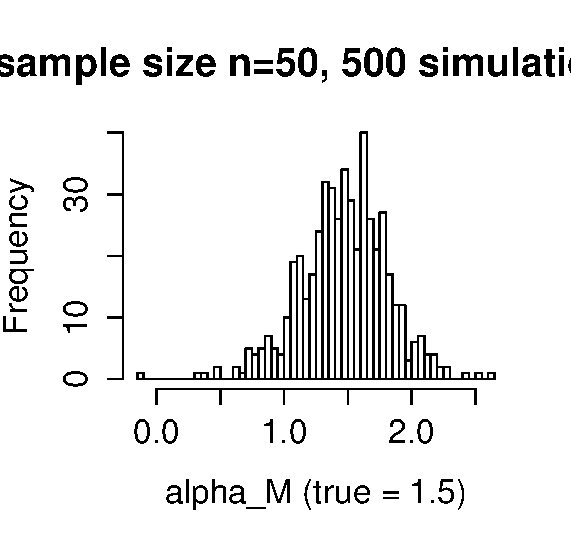
\includegraphics[scale=0.5]{alphaM50.pdf}&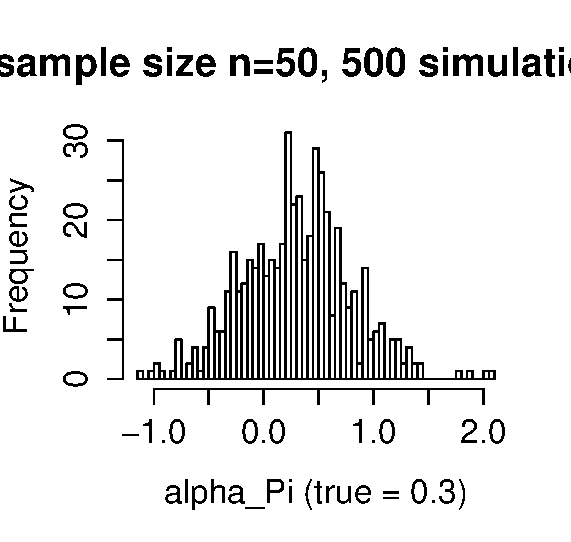
\includegraphics[scale=0.5]{alphapi50.pdf}&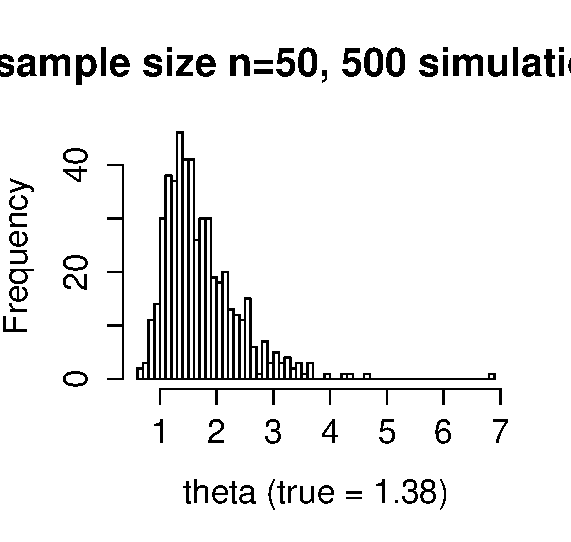
\includegraphics[scale=0.5]{theta50.pdf}\\
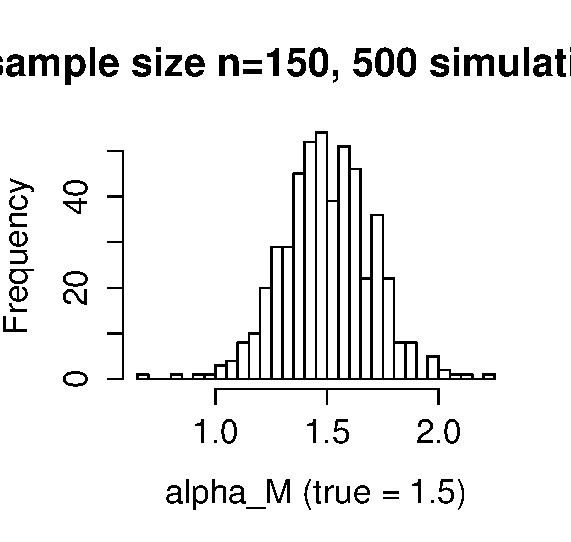
\includegraphics[scale=0.5]{alphaM150.pdf}&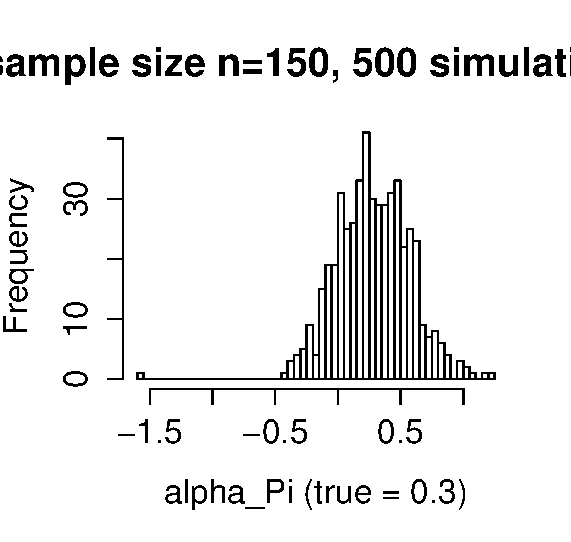
\includegraphics[scale=0.5]{alphapi150.pdf}&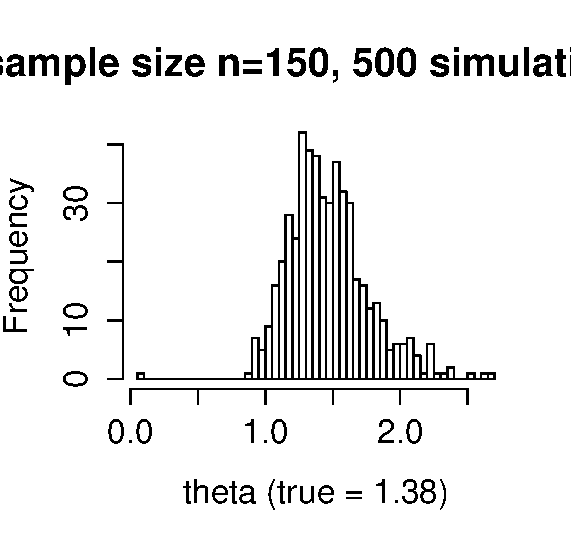
\includegraphics[scale=0.5]{theta150.pdf}\\
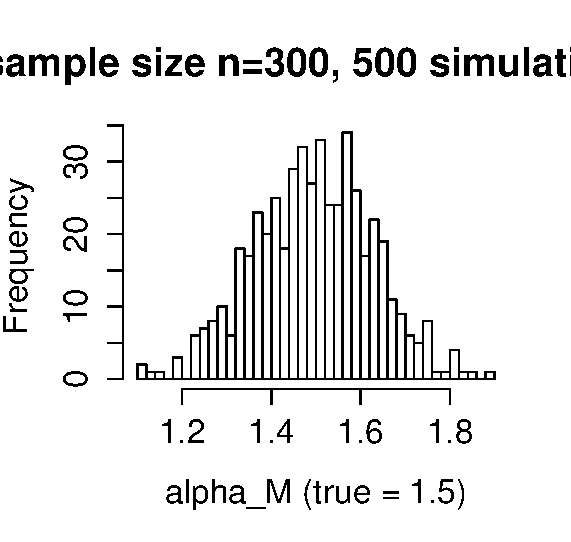
\includegraphics[scale=0.5]{alphaM300.pdf}&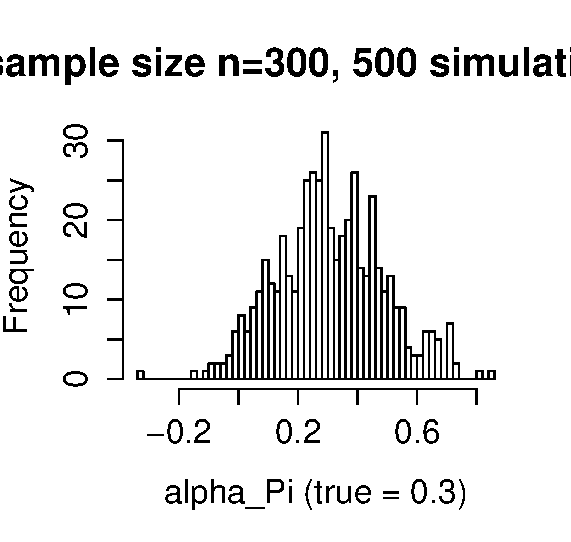
\includegraphics[scale=0.5]{alphapi300.pdf}&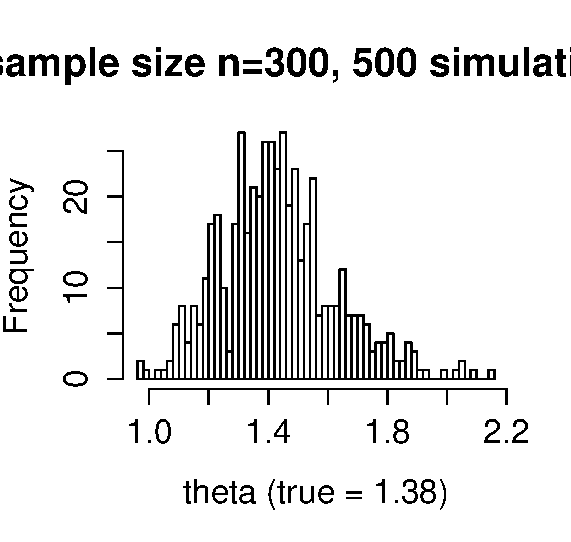
\includegraphics[scale=0.5]{theta300.pdf}\\
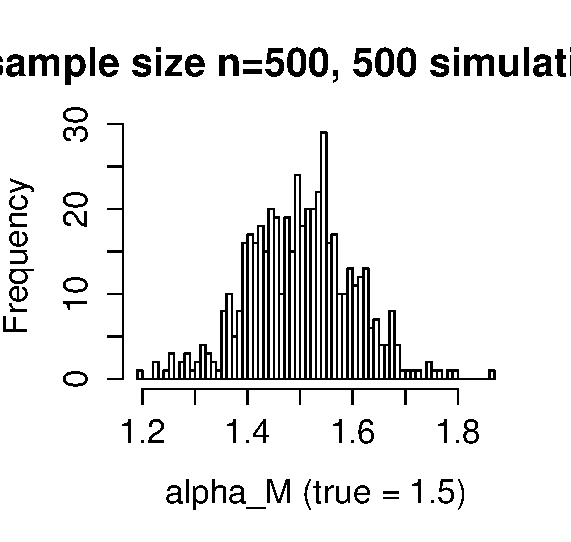
\includegraphics[scale=0.5]{alphaM500.pdf}&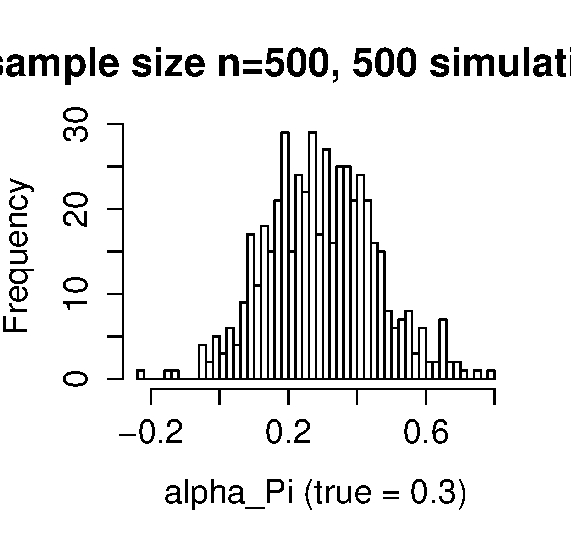
\includegraphics[scale=0.5]{alphapi500.pdf}&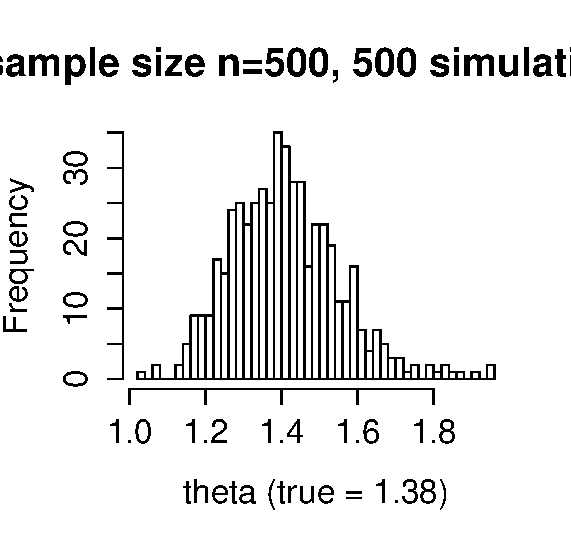
\includegraphics[scale=0.5]{theta500.pdf}
\end{tabular}



\end{document}